\documentclass[conference]{IEEEtran}

\usepackage{cite}
\usepackage{graphicx}
\usepackage{tikz}
\usepackage{pgfplots}
\usepackage{listings}
\usepgfplotslibrary{groupplots}
\usetikzlibrary{matrix}
\pgfplotsset{compat=newest}
\hyphenation{op-tical net-works semi-conduc-tor}

\usepackage{graphicx}
\graphicspath{ {images/} }

\begin{document}
\lstset{language=Java, basicstyle=\small, breaklines=true}



\title{Concurrent Patricia Trie \\ \normalsize https://github.com/kl4ng/concurrent-patricia-trie}

\author{\IEEEauthorblockN{Cole Garner}
\IEEEauthorblockA{School of Electrical Engineering and Computer Science\\
University of Central Florida\\
Orlando, Florida 32816\\
Email: ColeGarner@knights.ucf.edu}
\and
\IEEEauthorblockN{Kevin Lang}
\IEEEauthorblockA{School of Electrical Engineering and Computer Science\\
University of Central Florida\\
Orlando, Florida 32816\\
Email: klang@knights.ucf.edu}}

\maketitle


\begin{abstract}
This paper shows an implementation of a non-blocking Patricia Trie that combines techniques found in numerous recent implementations. It heavily uses the Compare and Swap operation and uses flags to prevent blocking. Additionally, it implements the flags in multiple locations in order to both increase efficiency and reduce the amount of conflicts. It also uses more efficient memory management and decreased overhead to improve upon its predecessors.
\end{abstract}


\section{Introduction}
A Patricia Trie, also known as a Radix tree, is a unique version of a regular tree. The defining feature of any trie, also known as a digital tree, is that the position of a node in a tree defines the key for that node. A Patricia trie takes this and optimizes the tree by merging any parent node with only one child in order to save space and create a more efficient tree.\cite{Shafiei2013} Because a Patricia Trie is a relatively simple data structure and has many practical uses, it is a good data structure to have an efficient parallelization technique for.
	
\begin{figure}[h]
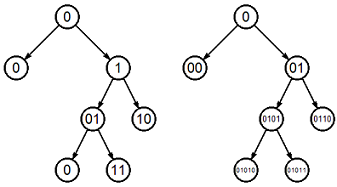
\includegraphics{patriciapreview}
\caption{An example of a Patricia Trie. The left diagram what is seen while transversing the tree and the right diagram shows what the full key value of each node is.}
\end{figure}

\par
Our implementation of a parallelized, lock-free Patricia Tree will aim to maximize performance and space-efficiency while removing some of the overhead of previous implementations by fine-tuning the memory management. We will combining multiple older approaches and taking the benefits of each and combining them. Our implementation will be focused on using compare-and-swap (CAS) operations which will allow for a blocking-free implementation. \cite{Shafiei2013,Brown2014}
\par
The main changes in our implementation from previous ones is that we will be storing the flags in multiple locations to allow for a smaller portion of the tree to be blocked off for some operations, creating less conflicts overall and increasing performance. \cite{Natarajan2014} The other main improvement we will be making is decreasing the overhead of creating and removing flags by compacting their size as much as possible, and more efficiently handling garbage collection .
\par
We originally planned to use a newer language called Rust to help our implementation by making use of its memory-safety property. However, we decided against this when we discovered that the language would not work in the way we wanted it to for our implementation.
\par
For the actual Patricia tree algorithm we will be using an algorithm similar to the pseudo-code seen in \cite{Shafiei2013}. However, we will be inserting various improvements on this algorithm, with the main one being that flags will also appear in the edges between two nodes to decrease conflicts. \cite{Natarajan2014}


\section{Related Works}
Creating high-performance, non-blocking data structures has advanced in recent years. There is work into making generalized data structures using CAS operations. \cite{Brown2013} This work has further been expanded into making generalized techniques for non-blocking trees. \cite{Brown2014} These techniques revolve around using load-link extended (LLX), store-conditional extended (SCX) and validate-extended (VLX) primitives which are generalized techniques of the standard, non-extended versions of the primitives. \cite{Brown2013, Brown2014} The techniques used are very powerful and efficient and help form a basis for some techniques used in our work.
\par
Earlier, non-generalized implementation of this technique was seen in a few different data structures. The one related to our work is Shafiei's implementation of non-blocking Patricia Tries. \cite{Shafiei2013} This implementation used a binary tree implementation and handled the parallization by creating flag objects for operations that keep track of what has to be changed. These flags are very powerful because they let multiple threads work on one operation so one thread is not forced to wait. Additionally, since the flag is there there is no chance of a portion of the tree becoming unusable if one thread fails in the middle of an operation. \cite{Shafiei2013, Howley2012} This technique is similar to ours, except we will be eliminating some of the overhead in their implementation due to the large amount of flags they created and the large size of each. Additionally we will be aiming to improve to memory management as compared to it.
\par
A slightly different work is an implementation of a lock-free binary search tree by Natarajan and Mittal. Their work also heavily involves CAS operations but the largest difference is that instead of marking the nodes they mark the edges between the nodes.\cite{Natarajan2014} This has interesting applications in that it allows a smaller portion of the tree to be flagged during insert and delete operations and allows for less conflicts on the whole.
\par
Similar to the previous work is another edge-based algorithm for a concurrent binary search tree by Ramachandran and Mittal. This is not a lock-free solution so it is not completely applicable to ours, however it involves edges and has relatively few nodes locked for each operation. \cite{Ramachandran2015} We will be using some of the techniques used here for the different operations to help further reduce the amount of nodes locked by other implementations and reduce the number of conflicts.
\par
Shun and Blelloch showed another alternative approach to parallization of trees with a multiway Cartesian tree. Theres is slightly unique in that they first create an array and then convert it into a tree. However, despite being different from out project, the algorithms they show in order to generate the tree from the array using parallization techniques warranted study. We looked into their techniques of differentiating what part a particular node is protected in, but ultimately decided the techniques were too far from our own to be much use. \cite{Shun2014}
\par
Due to us implementing this in a way with fully managed memory instead of utilizing a garbage collector, we will be utilizing hazard pointers as initially described by Michael in his seminal 2004 paper. \cite{Michael2004} While the original paper was more oriented towards C++, we will instead be modifying an existing implementation that was found publically available for Rust, extending and modifying it for our own use. \cite{CHAMT}

\section{Difficulties with Rust Language and Libraries}
Rust is a new programming language developed by Mozilla. Developed in parallel with their new Servo web rendering engine, it is developed from the ground up to support safety, concurrency, and parallelism, and was thus a very attractive candidate for our implementation of the concurrent patricia trie.\cite{MozillaResearch} Specifically, in terms of safety it guarantees no data races, buffer or stack overflow, and null pointer exceptions for most use cases. Due to its heavily static nature, it can validate the compiled program to be free of such errors and thus allows us to leverage this in creating a concurrent Patricia trie that has more simple aspects of memory management handled for us. Similarly, it is a language that focuses on speed, which will also help us achieve our desired result of having a Patricia trie implementation that out-performs its counterparts.
\par
However, Rust's approach to memory management, namely it being handled almost entirely by the language without a separate runtime for a garbage collector, has its limits. While this is true for most use cases, it becomes increasingly difficult for the compiler to guarantee this when the complexities of parallel lock-free algorithms come into play. The very nature of these algorithms relies more heavily on complex linearizability reasoning than the compiler can deduce, which means that more complex concurrency problems must have their own memory management, as is in our case.
\par
Do to, at the time, the alpha-stage status of the core language, in addition to our inexperience with the language, we ended up choosing to use Java instead. These difficulties included the fact that the main HazardPointer library we were intending to use did not even compile on the latest version of Rust\cite{CHAMT}. Due to the fact that we would have to manually do a large portion of our memory management by using unsafe constructs in Rust, the main advantages of the language disappeared with our use case. However, these difficulties led us to choose to implement a new algorithm (an edge-flagging patricia trie), instead of the original plan of simply doing a node-flagging patricia tree with managed memory.
\par


\section{Algorithm Description}
Our algorithm is devised from two state of the art techniques for concurrent trees both relying on CAS operations. The two techniques we will be using are the generalized non-blocking tree approach using flags inside nodes \cite{Shafiei2013,Brown2014} and the similar technique to have the flags be inside the edges instead of the nodes. \cite{Natarajan2014} By combining these two methods we will be able to take the advantages of both with some minor drawbacks.
\par
The main advantage to come the edge-based technique is that it allows for insert and delete operations to flag a smaller portion of the tree and use fewer atomic instructions. \cite{Natarajan2014} By doing this, the implementation will create fewer conflicts and will allow for more concurrent insert and delete operations, allowing for great speedups for trees with heavy emphasis on insert and delete. However, the method also causes seek operations to perform slightly worst sometimes by increasing the time it takes for them to reach their target node when there is a marked branch in their path. Because of this, we will combine this approach with the more traditional node-based approach for certain operations so that we can further improve the edge-based approach by only using it when necessary. 

Go into detail about what changes (if any) we make from the original pseudocode due to the nature of the Rust language (for better or for worse). Go into detail about what we do new (hopefully able to implement it with more than two children, or have less Flag objects).


\subsection{Data Structures}
The data structure used to store the Patricia Tree is simply a tree that stores a grand root node and a logical root node as well as all the functions to search and modify inside the tree. The two root structure is used for creating searching by forcing enough nodes to make a proper seek record. There is also a small data structure called SeekRecord used for storing a seekRecord during a seek operation.
\par
The individual node structure is also relatively simple. It contains a key to store for comparison purposes, which is technically unneeded due to the nature of a trie, but very helpful, as well as a mask which is used for. It contains a value and a mask, and perhaps the most important part is that instead of classic pointers to the children, it makes use of an AtomicStampedReference that allows for CAS operations on the edge between the two nodes and allows for both a node pointer and an integer to be stored. By allowing the integer to be stored inside the edge, it enables the edge to be flagged on the edge and is a large part of how our algorithm works.


\subsection{Algorithm}
The Patricia Trie initially contains a Grand root node linking to a dummy node and a logical root node. The logical root node will link to two dummy nodes representing. One of these represents all 0s, where the key is equal to 0, and the other represents all 1s, where the key is equal to the max value of an integer. With this the tree is created and we will now show you how the various operations will work on our algorithm.

\subsubsection{Get and Contains Operations}
These two operations are slightly different but accomplished in the same way. The operations work by starting at the logical root and going down the tree in much the same way that a normal trie would do it. The only unique feature here is that instead of using pointers, they are using the getReference function of the AtomicStampedReference.
\begin{lstlisting}[frame=lines]
pubic boolean contains(int key)
{
   return get(key) != null;
}

public T get(int key)
{
  Node node = rootNode;

  while(!isLeaf(node) && isPrefix(node,key))
  {
    if(node.key > key)
      node = node.left.getReference();
    else
      node = node.right.getReference();
   }

  if(isLeaf(node && key = node.key)
    return node.value;
  else
    return null;
}
\end{lstlisting}

\subsubsection{Insert Operation}
The insert operation is different from the previous two operations in that it is remarkably different from the linear version of the operation. This is one of the two operations that we implement that make use of the edge-based technique in order to implement the concurrency. 
\par
The algorithm for the operation is relatively simple. First it cycles through the tree storing the current and previous node until it either finds the node it is trying to insert, in which case it returns false, or the correct position for the node to be inserted. Once it has reached this part it then uses the current nodes key to generate the new key and mask for the new nodes. it then creates a new internal node and linkes it to both a new node that your inserting and the node originally in that position. Then at this point, it uses a CAS operation to ensure that the original node is still unchanged, and if it is, it then linkes the previous node to the new internal node which is linked to the new node and the original node. After this, the thread handles the cleanup.
\par
Because the CAS operation is done after the internal node is properly linked to everything, the operation is linearizble. From the view of other threads the entire operation takes place during the CAS and because of this, the operation is completely concurrent. And since we use the edge, no unrelated nodes are unavailble during the operation.

\begin{lstlisting}[frame=lines]
public boolean insert(int key, T value)
{
  Node node;
  Node prevNode;

  while(true)
  {
    prevNode = root;
    node = root.left.getReference();
      
    while(!isLeaf(node) && isPrefix(node,key))
    {
      prevNode = node;
      if(node.key > key)
        node = node.left.getReference();
      else
        node = node.right.getReference();
    }

    if(isLeaf(node) && node.key == key)
      return false;

    int bitwiseXOR = node.key ^ key;
    int counter = 0;
    while(bitwiseXOR != 0)
    {
      bitwiseXOR >>= 1;
      counter++;
    }

    int inKey = key >>> i << i;
    inKey = inKey | (1 << (i-1));
    int inMask = all1 >>> i << i;

    Node inter;
    Node newNode = new Node(key, value)
    if(node.key > key)
      inter = new Node(inkey,inMask,newNode,node)
    else
      inter = new Node(inkey,inMask,node,newNode)

    if(prevNode.key > key)
    {
      if(prevNode.left.compareAndSet(node,inter,Node.UF_UT,Node.UF_UT)
        return true;   
      else if(node == prevNode.left.getReference())
        cleanUp(key, seek(key));
    }
    else
    {
      if(prevNode.right.compareAndSet(node,inter,Node.UF_UT,Node.UF_UT)
        return true;   
      else if(node == prevNode.right.getReference())
        cleanUp(key, seek(key));
    }
  }
}
\end{lstlisting}

\subsubsection{Delete Operation}
Similar to the insert operation, the delete operation also takes advantage of the edge-based approach we are using. Unlike the insert operation, the delete operation has to keep track of multiple nodes to function correctly, and for this it uses both a seek record and the the grand root. 
\par
The delete operation functions by first getting the seek record which stores 4 nodes and then it uses a CAS operation to mark the edge from the parent to the node to be deleted and hadles the deletion and cleanup. This is once again linearizble because the entire deletion seems to take place during the CAS operation to other threads and since the cleanup only handles unreferenced nodes it is completely parallizible. 

\begin{lstlisting}[frame=lines]
public final void delete(int key)
{
  boolean isCleanup = false;
  SeekRecord<t> sRecord;
  Node parent;
  Node leaf = null;

  while(true)
  {
    sRecord = seek(key)
    if(!isCleanup)
    {
      leaf = sRecord.leaf;

      if(leaf.key != key)
        return;
      else
      {
        parent = sRecord.parent;
        if(parent.key > key)
        {
          if(par.left.compareAndSet(leaf,leaf,Node.UF_UT,Node.F_UT)
          {
            isCleanup = true;
            if(cleanUp(key, sRecord))
              return;
          }
          else if(leaf == parent.left.getReference())
            cleanUp(key, s);
        }
        else
        {
          if(par.right.compareAndSet(leaf,leaf,Node.UF_UT,Node.F_UT)
          {
            isCleanup = true;
            if(cleanUp(key, sRecord))
              return;
          }
          else if(leaf == parent.right.getReference())
            cleanUp(key, s);
        }
      }
    }

    else if(s.leaf == leaf)
    {
      if(cleanUp(key, s))
        return
    }

    else
      return;
  }
}
\end{lstlisting}

\section{Experimental Evaluation}
In this section, we will describe the results of evaluating our edge-based-flagging patricia trie with other similar concurrent data structures.

\subsection{Other Implementations}
The other data structures we will be using will be a lock-free binary search tree based on\cite{Natarajan2014} which is also implemented in Java\cite{LFBST}. The second and final data structure we will be testing our results with is a lock-free patricia trie with node-based flagging as described in\cite{Shafiei2013}. For the implementation, we reached out to the author who provided us with the Java source code of his non-replace implementation.

\subsection{Experimental Setup}
We conducted our experiments on a basic desktop computer with a 3.0GHz Q6600 Intel Quad Core, with 4GB of ram, and running the x86\_64 version of Fedora 21. As mentioned, all other implementations were also written in Java, and were executed under Java 8. Additionally, for those data structures that could accept any type of stored value, we made sure that this object was also an Integer, to minimize the difference object allocation/deallocation would have on the performance. Each simulation was run for a large enough number of iterations so that each test ran for approximately five seconds, and the results were then averaged and the throughput was calculated for each data point. For each test, we varied the following parameters, much in the same way as\cite{Natarajan2014}:

\begin{enumerate}
  \item \textbf{Key Range:} We varied the key range in order to test how the various data structures behaved under ranges of possible inserted values. We considered four different ranges: 1K, 10K, 100K, and 1M.
  \item \textbf{Operation Distribution:} Considering that performance of a data structure depends heavily on how often certain instructions were executed, we were sure to consider three different workload distributions. For the write dominated workload, we had 50\% insert and 50\% delete operations. For the mixed workload, we had 70\% search, 20\% insert, and 10\% delete. Lastly, the read dominated workload consisted of 90\% search, 9\% insert, and 1\% delete.
  \item \textbf{Number of Threads:} This varied the amount of contention in the data structure. We used the values of 1, 2, 4, 8, and 16.
\end{enumerate}

\subsection{Results}
As mentioned before, each simulation was run for around five seconds. The results are shown in Figure 1.
It is clear that the node-flagging implementation of the patricia trie (CPT-NODE-FLAG) has the best throughput for nearly every configuration, still performing better than our new edge-flagging implementation of the patricia trie (CPT-EDGE-FLAG). Another interesting data point is the fact that CPT-NODE-FLAG also outperformed the lock free binary search tree (BST-EDGE-FLAG) that uses the same edge-based flagging method as our implementation (CPT-EDGE-FLAG). Another important observation is the fact that our implementation has about equal throughput in comparison to the BST-EDGE-FLAG implementation, when averaged across all the configurations. 
\par
As the key range varies with the workload kept constant, there is no clear change in throughput for any of the algorithms, relatively speaking. However, a larger key range actually led to worse throughput, regardless of the workload type or number of threads. This can be seen in the graphs: in the write dominated configuration, e.g., there is a digression from around $7*10^6$ operations per second when at 8 threads at a 1K key range down to $1.4*10^6$ operations per second with the same amount of threads at a 1M key range.
\par
The difference between the differing workloads was also not very pronounced, in terms of relative performance. In terms of absolute performance of all the data structures, we saw that as we reduced the amount of write-oriented instructions, we saw an expected increase in throughput. One can look across any given row in Figure 2 in order to see that this is the case. For example, as we reduce the proportion of write instructions in the 1K key range, we see an improvement of max throughput from $7.5*10^6$ to $3*10^7$ operations per second, a fairly significant improvement. 


\subsection{Discussion}
The first thing that comes apparent when looking at the results is the similarity of throughput between BST-EDGE-FLAG and CPT-EDGE-FLAG (our implementation). This shows that the added checks performed at every branch during any seek within the patricia trie that are utilized to exit the search early have too much overhead to lead to significant throughput improvements over BST-EDGE-FLAG. Indeed, it shows that the added performance of being able to exit searching early equals the loss of performance that all those extra checks add.
\par
Additionally, its clear that CPT-NODE-FLAG, the node-based flagging method for the patricia trie, is the clear throughput winner in almost all configurations. This becomes more surprising when one looks at the results from other tests, such as in Natarajan and Mittal's\cite{Natarajan2014}, which found a clear improvement over node-based-flagging BST techniques. We speculate that this unexpected result is due to the nature of the Java runtime environment, where the excess amount of helper objects created by CPT-NODE-FLAG may not result in any loss of throughput due to the garbage collector never being called during the short time of our tests, for example. This may explain the discrepancy between our Java-based results and Natarajan and Mittal's C-based results. 
\par
Another possible explanation for these results is the possibility that the advantages of using edge-based flagging for a patricia trie are only more readily apparent in heavily parallel environment with 32 or more logical cores. Natarajan and Mittal's testing results\cite{Natarajan2014} seem to confirm this, as any significant improvements in throughput only become apparent with 16 or more threads within their 64 logical cores testing environment. 
\par

\begin{figure}
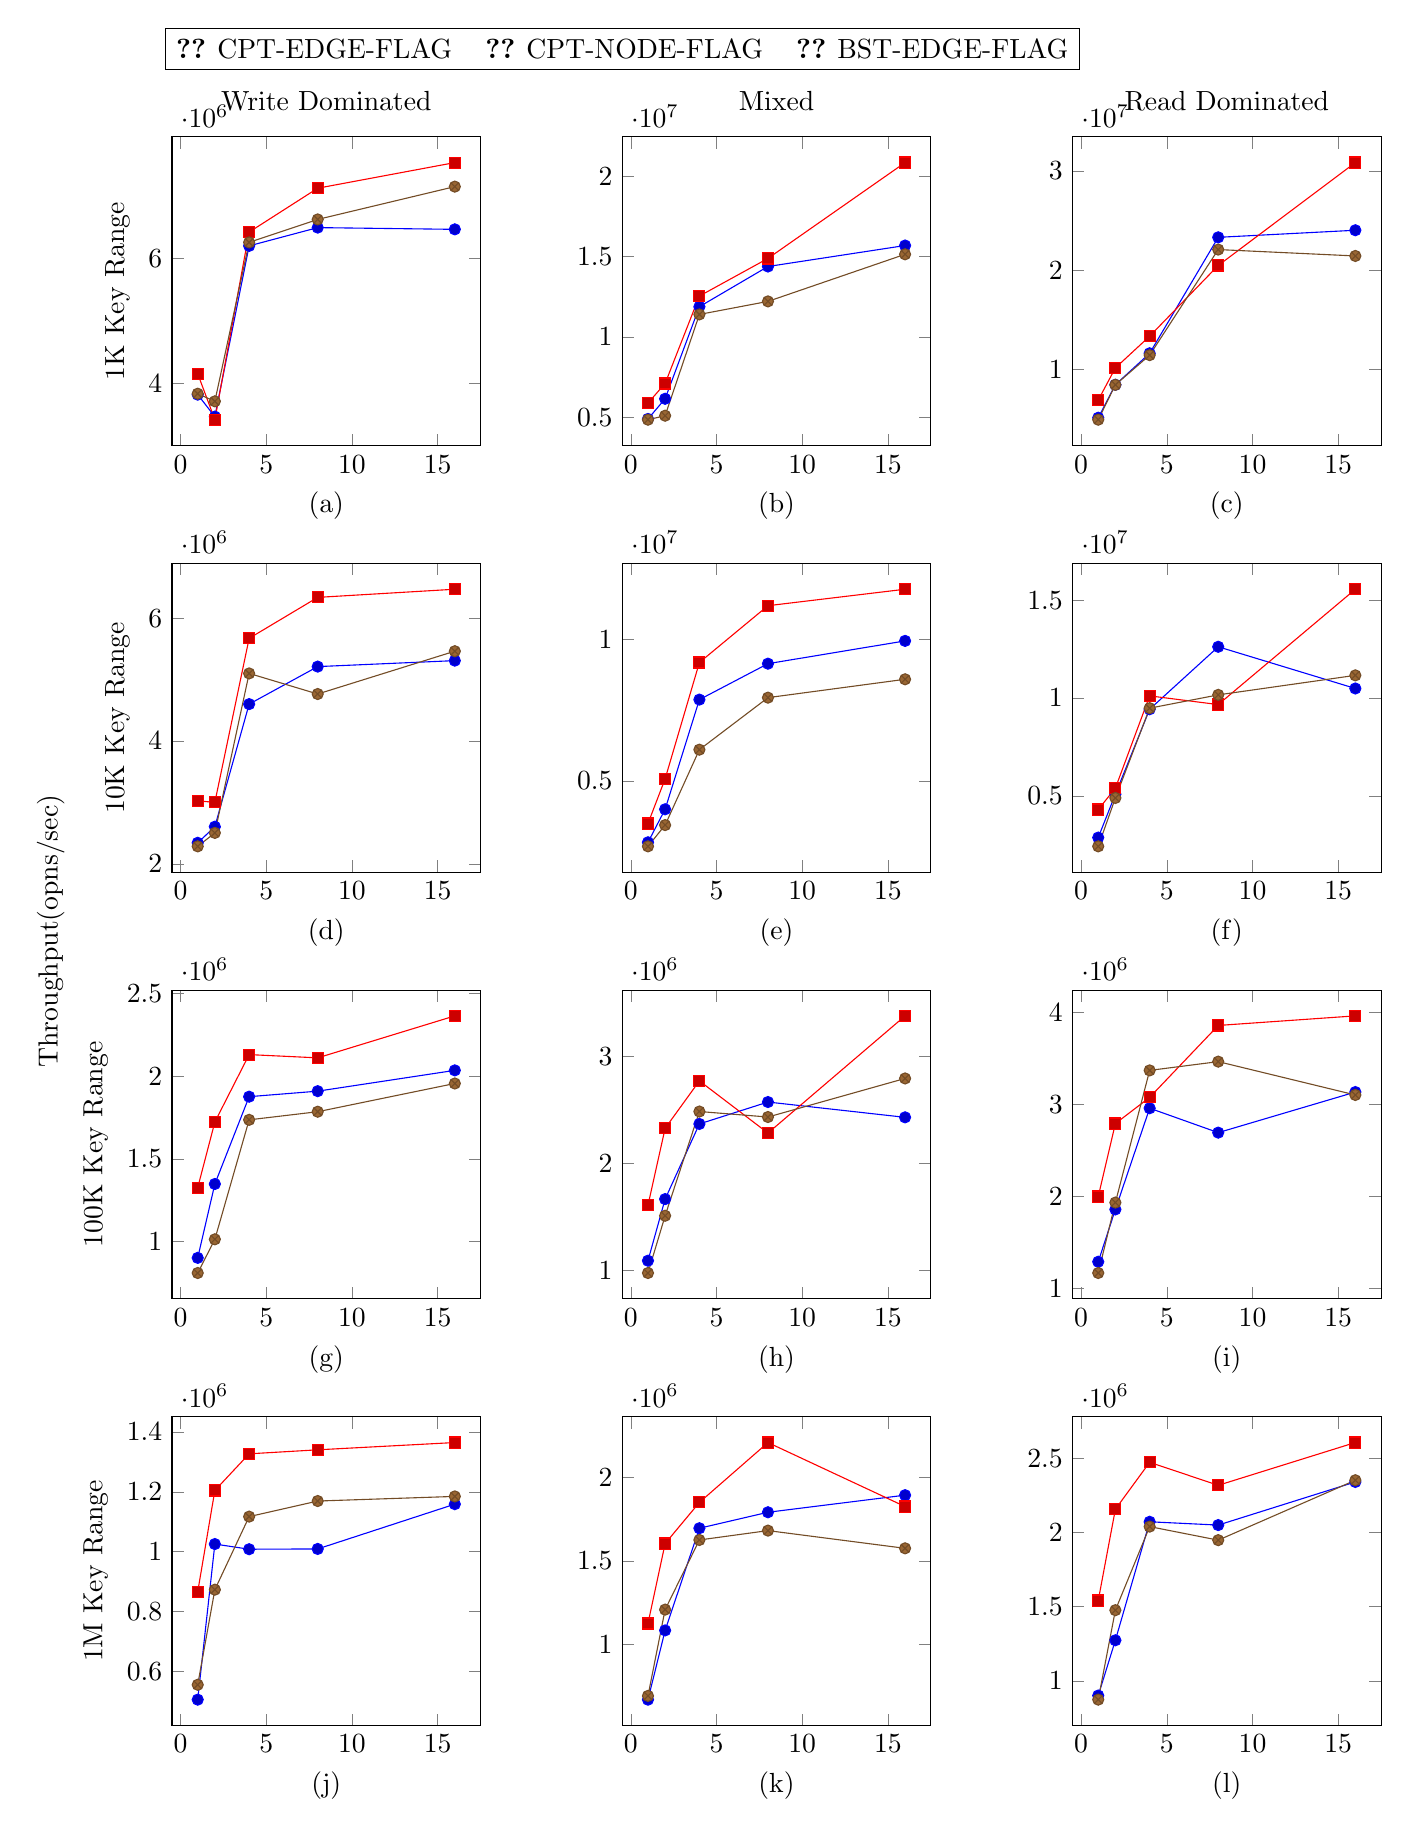
\begin{tikzpicture}
  \begin{groupplot}[group style={group size= 3 by 4, vertical sep=1.5cm, horizontal sep=1.8cm},height=5.5cm,width=5.5cm]
      
      %%
      % 0/50/50 1K
      \nextgroupplot[title=Write Dominated,xlabel={(a)},ylabel={1K Key Range}]
              \addplot coordinates {
                  (1, 3816793.893130) (2, 3463803.255975) (4, 6205398.696866) (8, 6498781.478473) (16, 6470921.297420)
              };\label{plots:cpt-ef}
              \addplot coordinates {
                  (1, 4152823.920266) (2, 3414134.516900) (4, 6426735.218509) (8, 7131395.970761) (16, 7542900.245144) 
              };\label{plots:cpt-nf}
              \addplot coordinates {
                  (1, 3831417.624521) (2, 3709198.813056) (4, 6261740.763932) (8, 6630200.563567) (16, 7156915.369476) 
              };\label{plots:bst-ef}
              \coordinate (top) at (rel axis cs:0,1);% coordinate at top of the first plot
      
      % 70/20/10 1K
      \nextgroupplot[title=Mixed,xlabel={(b)}]
              \addplot coordinates {
                  (1, 4892367.906067) (2, 6146281.499693) (4, 11876484.560570) (8, 14378145.219267) (16, 15683199.372672) 
              };\label{plots:cpt-ef}
              \addplot coordinates {
                  (1, 5882352.941176) (2, 7097232.079489) (4, 12539184.952978) (8, 14880952.380952) (16, 20844189.682126) 
              };\label{plots:cpt-nf}
              \addplot coordinates {
                  (1, 4844961.240310) (2, 5094243.504840) (4, 11396011.396011) (8, 12206286.237412) (16, 15137180.700095) 
              };\label{plots:bst-ef}
      
      % 90/9/1 1K
      \nextgroupplot[title=Read Dominated,xlabel={(c)}]
              \addplot coordinates {
                  (1, 5102040.816327) (2, 8431703.204047) (4, 11607661.056297) (8, 23310023.310023) (16, 24024024.024024) 
              };\label{plots:cpt-ef}
              \addplot coordinates {
                  (1, 6887052.341598) (2, 10131712.259372) (4, 13333333.333333) (8, 20470829.068577) (16, 30852294.639414) 
              };\label{plots:cpt-nf}
              \addplot coordinates {
                  (1, 4906771.344455) (2, 8424599.831508) (4, 11422044.545974) (8, 22075055.187638) (16, 21430484.864720) 
              };\label{plots:bst-ef}
      
      %%
      % 0/50/50 10K
      \nextgroupplot[ylabel={10K Key Range},xlabel={(d)}]
              \addplot coordinates {
                  (1, 2341920.374707) (2, 2604166.666667) (4, 4599816.007360) (8, 5210368.633581) (16, 5307503.483049)
              };\label{plots:cpt-ef}
              \addplot coordinates {
                  (1, 3024803.387780) (2, 3000300.030003) (4, 5670541.536717) (8, 6337135.614702) (16, 6469874.646179) 
              };\label{plots:cpt-nf}
              \addplot coordinates {
                  (1, 2284148.012791) (2, 2503128.911139) (4, 5099439.061703) (8, 4764173.415912) (16, 5461123.626186) 
              };\label{plots:bst-ef}
              
      % 70/20/10 10K
      \nextgroupplot[xlabel={(e)}]
              \addplot coordinates {
                  (1, 2842524.161455) (2, 4006410.256410) (4, 7870916.961826) (8, 9136592.051165) (16, 9939122.872407) 
              };\label{plots:cpt-ef}
              \addplot coordinates {
                  (1, 3503854.239664) (2, 5078720.162519) (4, 9178522.257916) (8, 11179429.849078) (16, 11759517.859768) 
              };\label{plots:cpt-nf}
              \addplot coordinates {
                  (1, 2699784.017279) (2, 3449465.332873) (4, 6106870.229008) (8, 7939658.594680) (16, 8586454.867447) 
              };\label{plots:bst-ef}
      
      % 90/9/1 10K
      \nextgroupplot[xlabel={(f)}]
              \addplot coordinates {
                  (1, 2873563.218391) (2, 5089058.524173) (4, 9429514.380009) (8, 12618296.529968) (16, 10489052.051921) 
              };\label{plots:cpt-ef}
              \addplot coordinates {
                  (1, 4306632.213609) (2, 5396654.074474) (4, 10111223.458038) (8, 9666505.558241) (16, 15558148.580319) 
              };\label{plots:cpt-nf}
              \addplot coordinates {
                  (1, 2426006.792819) (2, 4897159.647405) (4, 9483167.377904) (8, 10162601.626016) (16, 11159157.483610) 
              };\label{plots:bst-ef}
      
      %%
      % 0/50/50 100K
      \nextgroupplot[ylabel={100K Key Range},xlabel={(g)}]
              \addplot coordinates {
                                (1, 900252.070580) (2, 1347708.894879) (4, 1876700.760064) (8, 1910037.245726) (16, 2036037.870304)  
              };\label{plots:cpt-ef}
              \addplot coordinates {
                  (1, 1325556.733828) (2, 1723246.596588) (4, 2131514.441010) (8, 2111820.917586) (16, 2366023.896841) 
              };\label{plots:cpt-nf}
              \addplot coordinates {
                  (1, 808538.163001) (2, 1012658.227848) (4, 1736412.571627) (8, 1785554.861173) (16, 1956516.422510) 
              };\label{plots:bst-ef}
      
      % 70/20/10 100K
      \nextgroupplot[xlabel={(h)}]
              \addplot coordinates {
                  (1, 1087902.523934) (2, 1664447.403462) (4, 2367704.510477) (8, 2572678.157962) (16, 2429469.464606) 
              };\label{plots:cpt-ef}
              \addplot coordinates {
                  (1, 1606167.683906) (2, 2326663.564449) (4, 2770466.823660) (8, 2282323.405227) (16, 3378663.738491) 
              };\label{plots:cpt-nf}
              \addplot coordinates {
                  (1, 972762.645914) (2, 1508523.155830) (4, 2483854.942871) (8, 2432350.258437) (16, 2793296.089385) 
              };\label{plots:bst-ef}
              
      % 90/9/1 100K
      \nextgroupplot[xlabel={(i)}]
              \addplot coordinates {
                  (1, 1287001.287001) (2, 1855976.243504) (4, 2956393.200296) (8, 2690884.628322) (16, 3132096.155352) 
              };\label{plots:cpt-ef}
              \addplot coordinates {
                  (1, 1996007.984032) (2, 2789400.278940) (4, 3074085.459576) (8, 3856165.043864) (16, 3960396.039604) 
              };\label{plots:cpt-nf}
              \addplot coordinates {
                  (1, 1164958.061510) (2, 1930501.930502) (4, 3367570.298030) (8, 3462903.644706) (16, 3100414.680464) 
              };\label{plots:bst-ef}
      
      %%
      % 0/50/50 1M
      \nextgroupplot[ylabel={1M Key Range},xlabel={(j)}]
              \addplot coordinates {
                                (1, 504948.495253) (2, 1025325.540859) (4, 1008013.708986) (8, 1008954.470929) (16, 1158731.768080) 
              };\label{plots:cpt-ef}
              \addplot coordinates {
                  (1, 865650.969529) (2, 1204529.029150) (4, 1327051.954084) (8, 1340482.573727) (16, 1364815.067558) 
              };\label{plots:cpt-nf}
              \addplot coordinates {
                  (1, 554692.700244) (2, 872752.661896) (4, 1117068.811439) (8, 1169180.404536) (16, 1184641.127778) 
              };\label{plots:bst-ef}

      % 70/20/10 1M
      \nextgroupplot[xlabel={(k)}]
              \addplot coordinates {
                  (1, 671140.939597) (2, 1084951.719648) (4, 1695489.996609) (8, 1790911.126035) (16, 1893132.661271) 
              };\label{plots:cpt-ef}
              \addplot coordinates {
                  (1, 1126126.126126) (2, 1603849.238172) (4, 1849796.522383) (8, 2207505.518764) (16, 1824942.400255) 
              };\label{plots:cpt-nf}
              \addplot coordinates {
                  (1, 693673.695893) (2, 1209189.842805) (4, 1625355.546526) (8, 1681308.057669) (16, 1575454.420134) 
              };\label{plots:bst-ef}
      
      % 90/9/1 1M
      \nextgroupplot[xlabel={(l)}]
              \addplot coordinates {
                  (1, 900414.190528) (2, 1273398.701133) (4, 2072753.653228) (8, 2050545.957861) (16, 2341577.637934) 
              };\label{plots:cpt-ef}
              \addplot coordinates {
                  (1, 1541307.028360) (2, 2157497.303128) (4, 2474022.761009) (8, 2318840.579710) (16, 2607476.940126) 
              };\label{plots:cpt-nf}
              \addplot coordinates {
                  (1, 873057.447180) (2, 1476450.612727) (4, 2040191.778027) (8, 1948842.874543) (16, 2353079.592917) 
              };\label{plots:bst-ef}
              \coordinate (bot) at (rel axis cs:0,0);% coordinate at bottom of the last plot
  \end{groupplot}
  
  \path (top-|current bounding box.west)-- 
        node[anchor=south,rotate=90] {Throughput(opns/sec)} 
        (bot-|current bounding box.west);
          
  % legend
  \path (top|-current bounding box.north)--
        coordinate(legendpos)
        (bot|-current bounding box.north);
  \matrix[
      matrix of nodes,
      anchor=south,
      draw,
      inner sep=0.2em,
      draw
    ]at([yshift=1ex]legendpos)
    {
      \ref{plots:cpt-ef}& CPT-EDGE-FLAG&[8pt]
      \ref{plots:cpt-nf}& CPT-NODE-FLAG&[8pt]
      \ref{plots:bst-ef}& BST-EDGE-FLAG\\};
\end{tikzpicture}
\caption{Each row represents a different key range. Each column, a workload type.}
\end{figure}
\clearpage


\section{Conclusion and Future Work}
In this paper, we present a new lock-free algorithm for concurrent manipulation of a binary patricia trie that uses compare-and-swap and bit-test-and-set atomic instructions. While our algorithm does not out-perform the node-flagging implementation that we sought to improve upon, it does have its own advantages that may be more evident in a non-garbage-collected environment.
\par
Further work to be done consists of implementing this algorithm in a managed memory environment (such as C) and see the degree to which that affects the throughput relative to the algorithms described in\cite{Shafiei2013}\cite{Natarajan2014}. Additionally, the performance difference between ours and other similar algorithms should be tested within a more parallel environment to see how it performs comparatively within a highly parallel testing environment. Other future work includes adding a replace operation to our algorithm and comparing the ease of implementation and performance of that with a node-flagging patricia trie that also implements a replace operation\cite{Shafiei2013}.


\section{Acknowledgment}
We would like to thank Niloufar Shafiei for providing her source code for her Java implementation of her paper's algorithm\cite{Shafiei2013} and her willingness to help us. We would also like to thank Arunmoezhi Ramachandran for his publicly available Java implementation of lock free binary search trees with edge-based-locking\cite{LFBST}.


% references section
\bibliographystyle{IEEEtran}
\bibliography{IEEEabrv,references}


\end{document}
